\documentclass{article}
\usepackage{graphicx} % Required for inserting images
\usepackage{graphicx} % Required for inserting images
\usepackage[brazil]{babel}
\usepackage[utf8]{inputenc} %Pacote para acentuação
\usepackage[lmargin=3cm,tmargin=3cm,rmargin=2cm,bmargin=2cm]{geometry} %Formato que lembra a ABNT
\usepackage[T1]{fontenc} %Ajusta o texto que vem de outras fontes
\usepackage{amsmath,amsthm,amsfonts,amssymb,dsfont,mathtools,blindtext} %pacotes matemática
\usepackage{multicol} % Allows for multiple columns


\begin{document}

\begingroup % Create the command for including the title page in the document
\hbox{ % Horizontal box
\hspace*{0.2\textwidth} % Whitespace to the left of the title page
\rule{1pt}{\textheight} % Vertical line
\hspace*{0.05\textwidth} % Whitespace between the vertical line and title page text
\parbox[b]{0.75\textwidth}{ % Paragraph box which restricts text to less than the width of the page
{\noindent\Huge\bfseries Trabalho de Matemática \\}\\[2\baselineskip] % Title
{\large \textit{\textbf{Nome:} Pedro Jorge de Souza Colombrino  \ \ \ \\ \textbf{RA:} 0051352311015 \ \ \ \ \textbf{Curso:} Ciência de Dados }}\\
[1\baselineskip]
{\large \textbf{Tema:} Determinante } \\[4\baselineskip] % Tagline or further description
{\large \textsc{ Alexandre Garcia de Oliveira

}} 

\vspace{0.5\textheight} % Whitespace between the title block and the publisher
{\noindentFaculdade Faculdade de Tecnologia da Baixada Santista Rubens Lara }\\[\baselineskip] % Publisher and logo
}}
\endgroup

1. Deduza o determinante de uma matriz $4\times4$:

\begin{equation}
A = \begin{bmatrix}
a_{11} & a_{12} & a_{13} & a_{14} \\
a_{21} & a_{22} & a_{23} & a_{24} \\
a_{31} & a_{32} & a_{33} & a_{34} \\
a_{41} & a_{42} & a_{43} & a_{44} \\
\end{bmatrix}
\end{equation}


\begin{aligned}
\det(A) &= \sum_{\sigma \in S_4} (\operatorname{sgn}(\sigma)) \prod_{i=1}^{4} a_{i,\sigma(i)} \\

&= a_{1,1} a_{2,2} a_{3,3} a_{4,4} - a_{1,1} a_{2,2} a_{3,4} a_{4,3} - a_{1,1} a_{2,3} a_{3,2} a_{4,4}  
+ a_{1,1} a_{2,3} a_{3,4} a_{4,2} + a_{1,1} a_{2,4} a_{3,2} a_{4,3} - a_{1,1} a_{2,4} a_{3,3} a_{4,2} 
- a_{1,2} a_{2,1} a_{3,3} a_{4,4} + a_{1,2} a_{2,1} a_{3,4} a_{4,3} + a_{1,2} a_{2,3} a_{3,1} a_{4,4} 
&- a_{1,2} a_{2,3} a_{3,4} a_{4,1}  - a_{1,2} a_{2,4} a_{3,1} a_{4,3} + a_{1,2} a_{2,4} a_{3,3} a_{4,1} 
+ a_{1,3} a_{2,1} a_{3,2} a_{4,4} - a_{1,3} a_{2,1} a_{3,4} a_{4,2} - a_{1,3} a_{2,2} a_{3,1} a_{4,4} 
+ a_{1,3} a_{2,2} a_{3,4} a_{4,1} &+ a_{1,3} a_{2,4} a_{3,1} a_{4,2} - a_{1,3} a_{2,4} a_{3,2} a_{4,1} 
- a_{1,4} a_{2,1} a_{3,2} a_{4,3} + a_{1,4} a_{2,1} a_{3,3} a_{4,2} + a_{1,4} a_{2,2} a_{3,1} a_{4,3} 
- a_{1,4} a_{2,2} a_{3,3} a_{4,1} &- a_{1,4} a_{2,3} a_{3,1} a_{4,2} + a_{1,4} a_{2,3} a_{3,2} a_{4,1}\\ 
\\
\\
\\
\\
\end{aligned}
2.  Calcule o determinante, usando o que foi deduzido, de duas matrizes definidas pelo autor. Considere uma matriz A cujo det(A) = 0 e outra matriz B cujo det(V) \neq 0.}\\
\\

Matriz de det(A) = 0 
\begin{equation}
A = \begin{bmatrix}
8 & 8 & 8 & 8 \\
8 & 8 & 8 & 8 \\
8 & 8 & 8 & 8 \\
0 & 0 & 0 & 0 \\

\end{bmatrix}
\end{equation} 
\\
&= (8*8*8*0) - (8*8*8*0) - (8*8*8*0)+ (8*8*8*0) + (8*8*8*0) - (8*8*8*0)
- (8*8*8*0) +(8*8*8*0) + (8*8*8*0) &- (8*8*8*0)  - (8*8*8*0) +  (8*8*8*0)
+  (8*8*8*0) -  (8*8*8*0) -  (8*8*8*0) +  (8*8*8*0) &+  (8*8*8*0) - (8*8*8*0)
-  (8*8*8*0) +  (8*8*8*0) +  (8*8*8*0) -  (8*8*8*0) &-  (8*8*8*0) +  (8*8*8*0) = 0\\ 

det(A) = 0, pois se uma matriz tem uma linha ou uma coluna inteira com elementos iguais a zero, então o determinante dessa matriz será igual a zero.\\
\\

\\


Matriz de det(B)\neq 0 

\begin{equation}
B = \begin{bmatrix}
4 & 0 & 0 & 0 \\
0 & 4 & 0 & 0 \\
0 & 0 & 4 & 0 \\
0 & 0 & 0 & 4 \\
\end{bmatrix}
\end{equation}
\\

&= (4*4*4*4) - (4*4*4*0) +  (4*0*0*4) + (4*0*0*0) + (4*0*0*0)- (4*0*4*0)
-(0*0*4*4) + (0*0*0*0) +(0*0*0*4) - (0*0*0*0) - (0*0*0*0) + (0*0*4*0) 
+ (0*0*0*4) - (0*0*0*0) -(0*4*0*4) + (0*4*0*0) + (0*0*0*0) - (0*0*0*0)
-(0*0*0*0) +(0*0*4*0) +(0*4*0*0) - (0*4*4*0) - (0*0*0*0) + (0*0*0*0) = 256\\  
\\
  O determinante de uma matriz diagonal é igual ao produto dos elementos na diagonal principal. Neste caso, todos os elementos na diagonal principal são iguais a 4, então o determinante é:\\

det(B) = 4*4*4*4 = 256 \\





\section*{Código em python:}

\begin{figure}[ht] 
    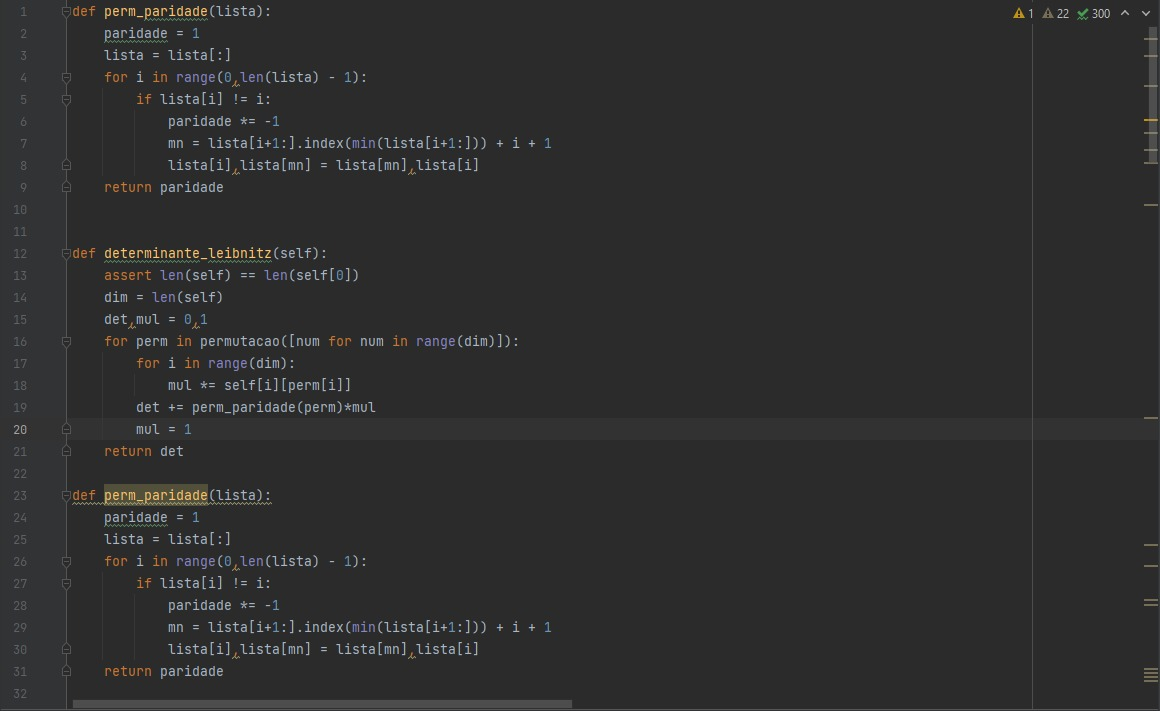
\includegraphics[width=12cm]{1.jpeg}   
\end{figure}
\begin{figure}[ht] 
    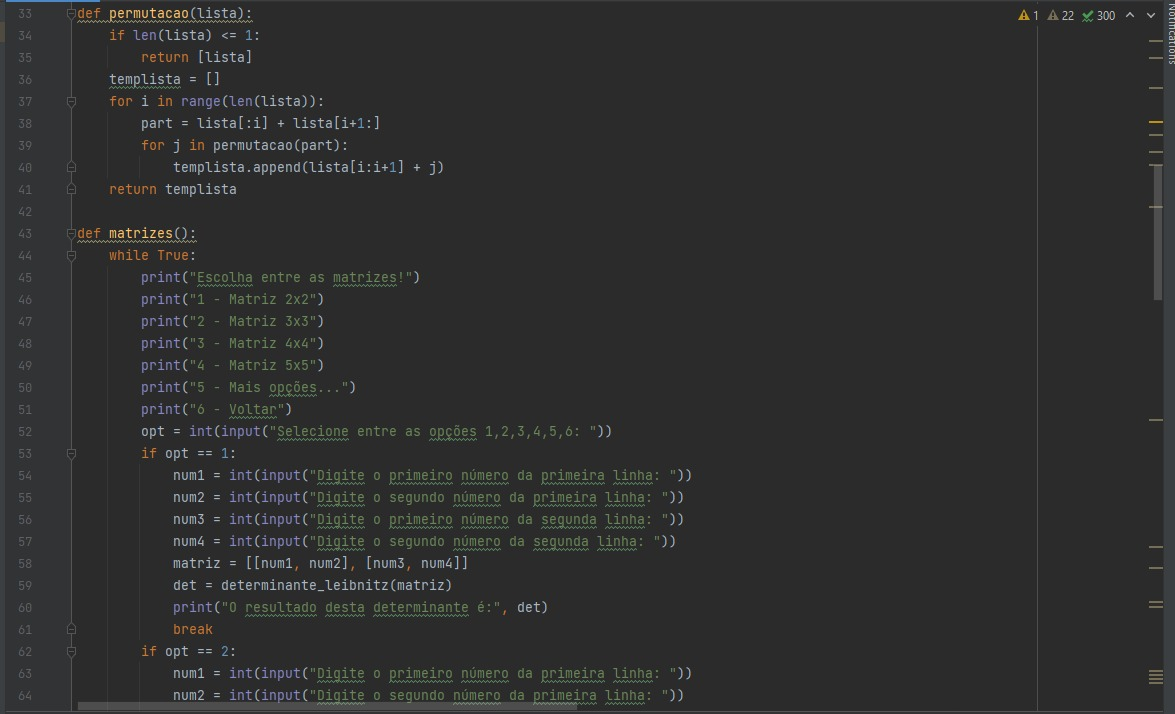
\includegraphics[width=12cm]{2.jpeg}   
\end{figure}
\begin{figure}[ht] 
    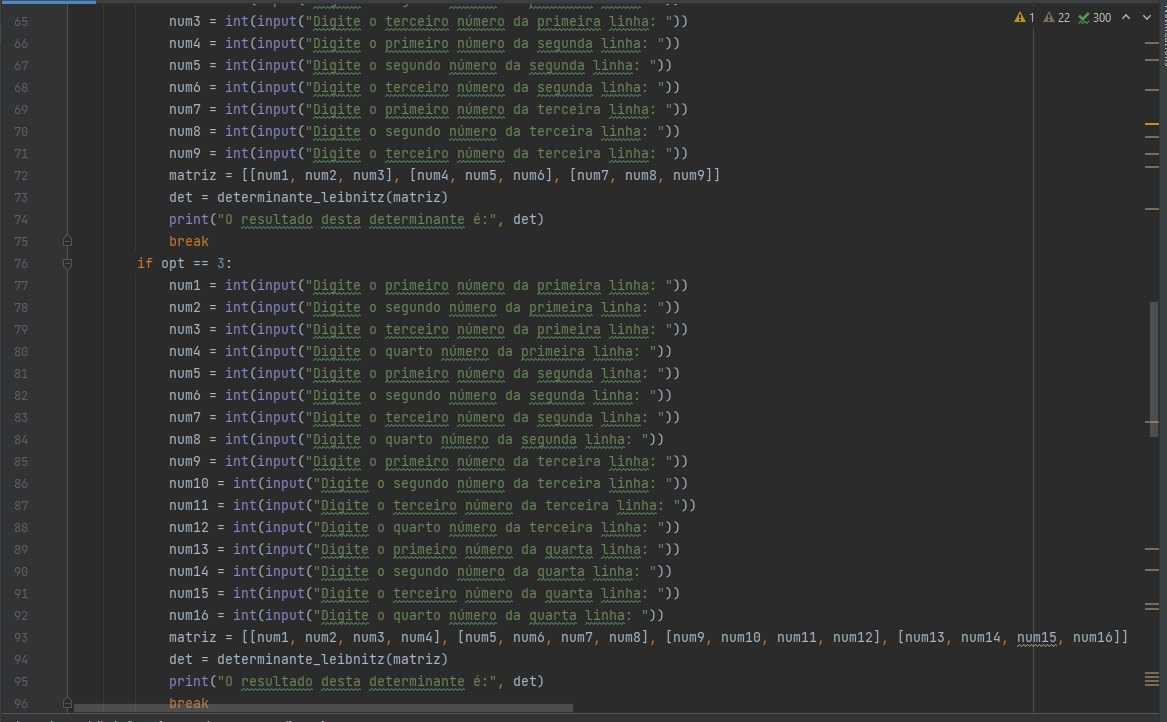
\includegraphics[width=12cm]{3.jpeg}   
\end{figure}
\begin{figure}[ht] 
    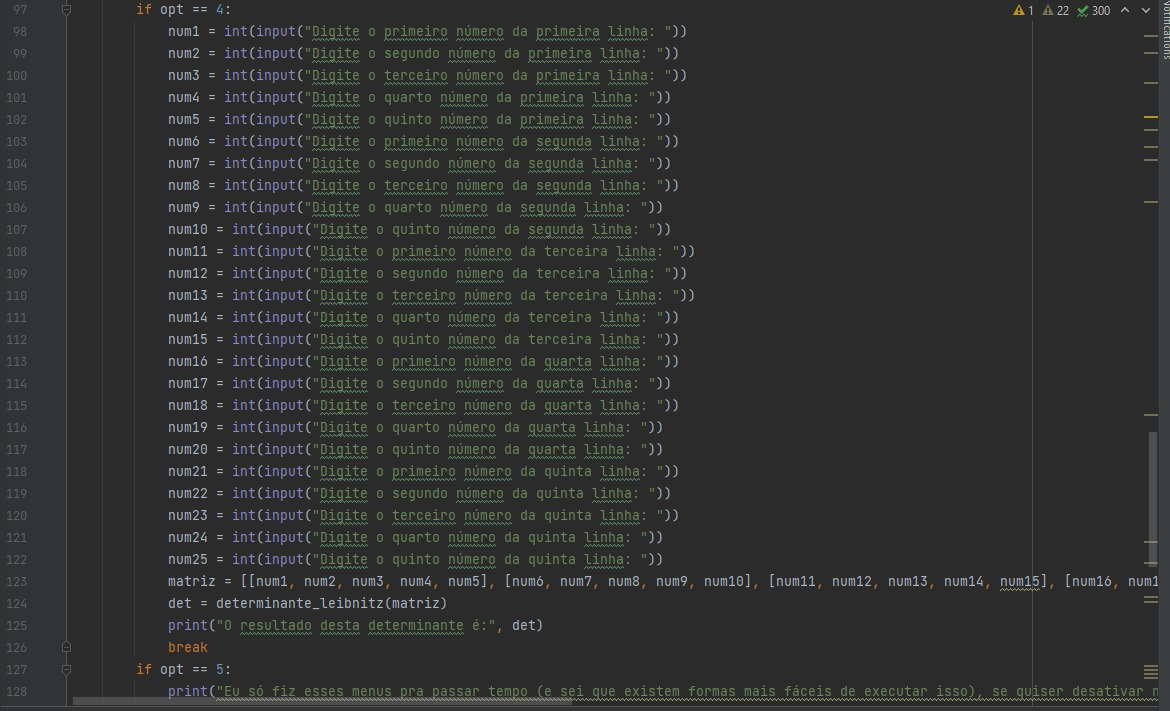
\includegraphics[width=12cm]{4.jpeg}   
\end{figure}
\begin{figure}[ht] 
    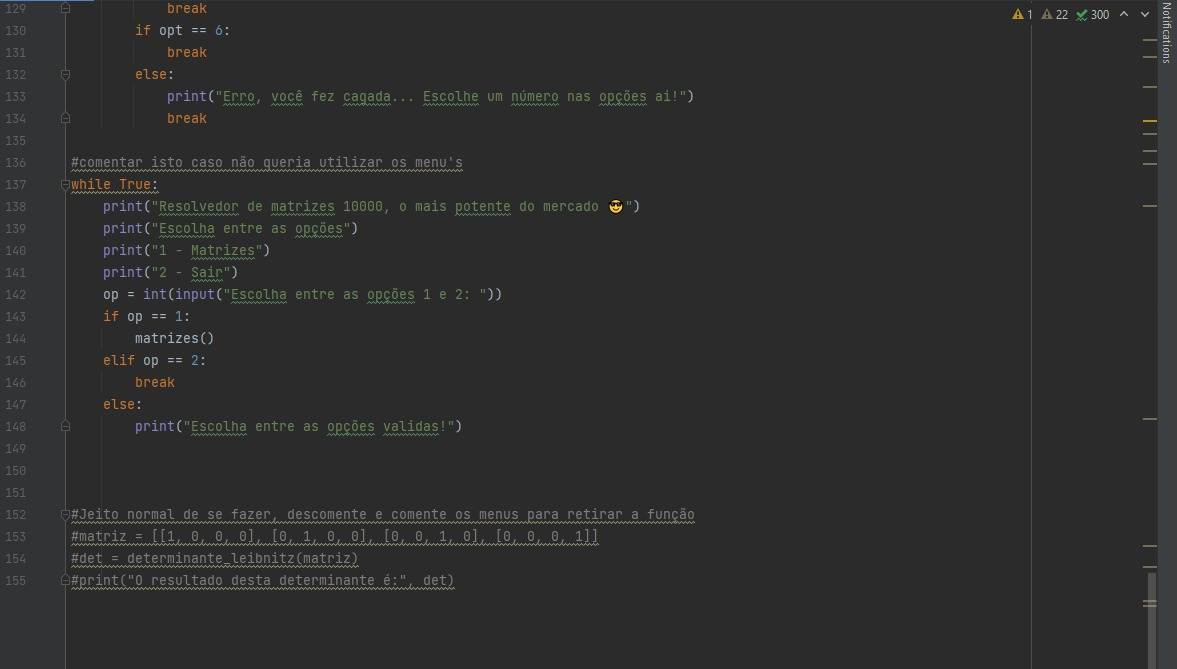
\includegraphics[width=12cm]{5.jpeg}   
\end{figure}
\begin{figure}[ht] 
    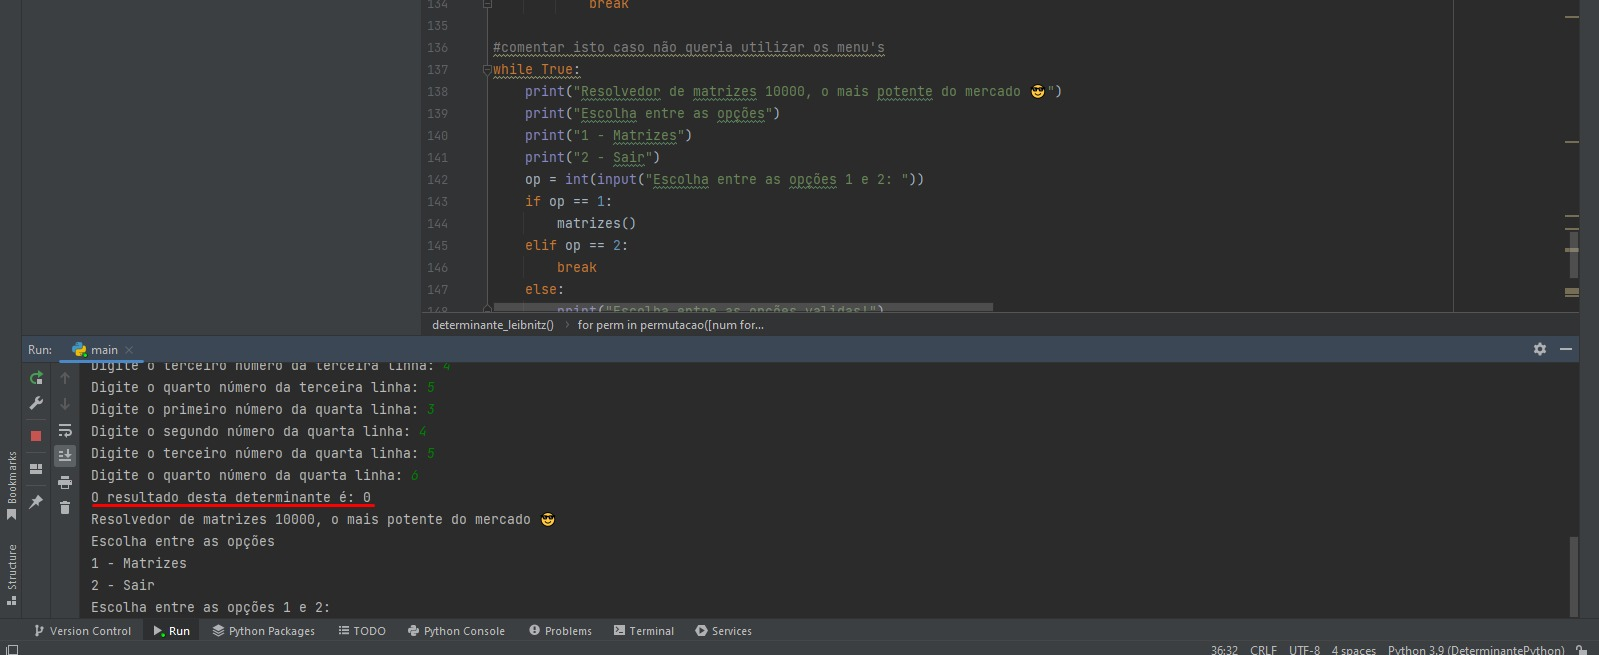
\includegraphics[width=12cm]{6.jpeg}   
\end{figure}
\begin{figure}[ht] 
    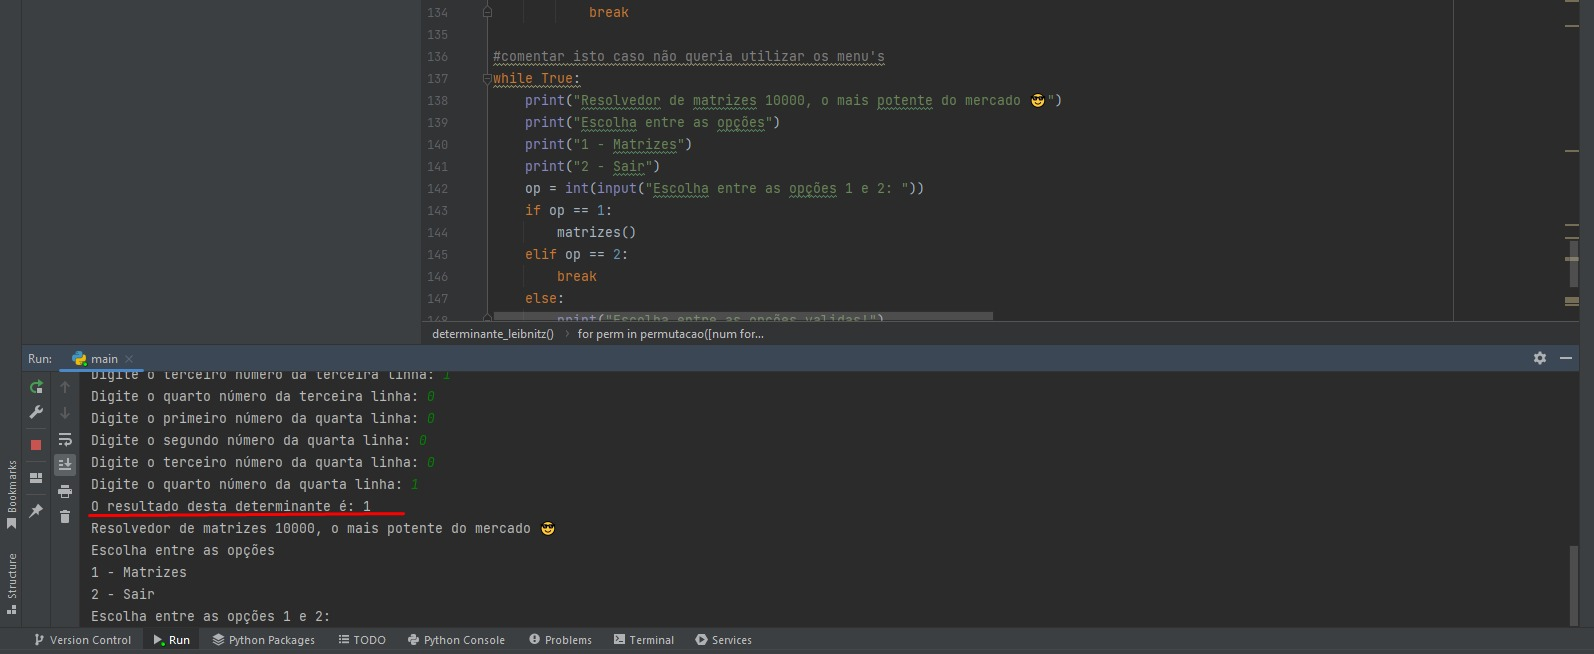
\includegraphics[width=12cm]{7.jpeg}   
\end{figure}
\end{document}
